\documentclass{article}
\usepackage[utf8]{inputenc}
\usepackage{graphicx}
\usepackage{blindtext}
\usepackage{subfiles}
\usepackage[colorlinks = false]{hyperref}
\usepackage[table]{xcolor}
\usepackage{rotating}

\usepackage[TS1,T1]{fontenc}

\usepackage[
backend=biber,
style=authoryear,
citestyle=authoryear
]{biblatex}
\renewcommand*{\bibfont}{\footnotesize}
\usepackage[normalem]{ulem}
\usepackage{fancyhdr}
\pagestyle{fancy}
\fancyhf{}
\rhead{Measuring Rhetorical Similarity}
\lhead{Nicolai Berk}
\cfoot{\thepage}

\useunder{\uline}{\ul}{}

\addbibresource{refs.bib}

\title{Measuring Rhetorical Similarity with Supervised Machine Learning
\footnote{Replication materials are available via \href{https://github.com/nicolaiberk/SMLSE}{https://github.com/nicolaiberk/SMLSE}}
}
\author{Nicolai Berk}
\date{\today}


\begin{document}

% - Heinz-Christian Strache

% - Sebastain Kurz

% quotes should show obvious similarities

\maketitle

\begin{abstract}
Political scientists are often interested in the rhetorical similarity of different sets of texts. Despite the centrality of the measurement of rhetorical similarities to political science research, common approaches are limited. Building on the idea that text classifiers' predicted probabilities are substantive similarity estimates, I propose a supervised machine learning similarity estimate (SMLSE) to measure the similarity of a given document with a specified corpus. It is able to a) assess underlying dimensions distinguishing a corpus from other documents and b) provide a precise similarity estimate for each document. The paper outlines a best practice that researchers should follow in the application of this approach. Showcasing data from parliamentary speeches from four case studies in Austria, Germany, and the Netherlands, I provide evidence that this process produces valid estimates of parties' and individuals' similarities with the radical-right. Evidence is presented that SMLSEs provide more precise results than existing state-of-the-art approaches.\par \medskip

\textbf{Keywords:} Rhetorical similarity, text analysis, supervised learning, machine learning, party competition, radical-right, political rhetoric.
\end{abstract}



\section{Introduction}
\label{sec:Intro}
Political scientists are often interested in the rhetorical similarity of different sets of texts. For example, scholars of representation might be interested whether certain groups communicate distinctively in parliament (\cite{Pitkin1967}) or whether legislation is similar to demands voiced by interest groups (\cite{Kluver2019}). Students of government formation and termination want to know which parties communicate most similar and are hence most likely to govern with each other and how stable these coalitions might be (\cite{Gamson1961, Grofman1994}), or whether coalitions increase the similarity of parties over time (\cite{Spoon2019}). Public opinion scholars evaluate which political groups left their mark on the current public discourse (\cite{Wagner2017, Slothuus2010k}). Scientists interested in party competition might assess historical similarities between parties to judge whether one party filled a place abandoned by another (\cite{Kitschelt1986}), or whether one party moved towards another (\cite{Downs1957, Meguid2005b}). Knowing how similar MPs communicate allows to judge whether certain MPs are likely to leave their party (\cite{Hirschman1970}) or which direction the party might take if specific MPs took over leadership of the party (\cite{Fernandez-Vazquez2016}).\par

Despite the centrality of rhetorical similarities to political science research, existing approaches to measure it are limited. Scaling methods such as wordscore (\cite{Laver2003}) and wordfish (\cite{Slapin2008}) place labels\footnote{I define 'labels' as meta-information about documents (such as authorship), which allows to group said documents into corpora. A corpus (plural: corpora) is a group of documents.} in a one- (wordfish) or multi-dimensional space (wordscore), based on their word usage. These measures were designed for measuring ideological positions, not similarities, as they cannot precisely estimate the similarity of a given document \textit{with} a corpus. Simpler similarity measures, such as cosine similarity, are designed to assess literal identity of single documents, however perform badly for meaningful assessments (\cite{Prasetya2018}). To my knowledge, no specified method to estimate the rhetorical similarity of groups exists at the time of writing.\par

To address this methodological gap, I propose a \textit{supervised machine learning similarity estimate} (SMLSE) to measure the similarity of a given document with a specified corpus. This approach builds on an existing method to assess the similarity between groups using classifier accuracy (\cite{Peterson2018}), but moves beyond it by focussing on predicted probabilities. This enables to provide a precise similarity estimate for each document, based on its word use. The next section briefly reviews existing methods to estimate similarities before presenting this new approach and explaining how to estimate SMLSEs step by step. Using parliamentary speeches from Austria, Germany, and the Netherlands, I then provide evidence indicating that the estimates are able to distinguish radical-right parties in line with theoretical expectations and produce valid estimates of similarity to the radical-right for parties and speakers. The last section compares SMLSEs with wordfish and cosine similarity estimates and shows that the method returns more meaningful and precise results.\par


\section{Estimating rhetorical similarity}

A measure of rhetorical similarity should have several properties to be considered valid and useful. First, such an indicator should reflect a given document's similarity to other documents. The resulting estimate should then be informative about which corpus a document is likely to belong to. As textual data sets are often very large, the method should be scalable and fast to apply. Ideally, it's application would not presuppose an understanding of the language through the researcher, but allow for 'language-blind' application in different contexts. However, \textit{if} the researcher is able to understand the language, meaningful information about what drives similarities and distinctiveness of documents is desirable. \par


\subsection{Existing similarity measures}

Several existing methods could be used to measure rhetorical similarity. One of the most popular methods - cosine similarity - places documents in a multidimensional space. Every word constitutes a dimension and the number of times that word was used defines the placement of a document on that dimension. Each document is then represented by a vector in high-dimensional (word) space. The cosine of the angle between those two vectors indicates how similar the word use in two given documents is, independent of the documents' length\footnote{That is, two documents containing words $a$ and $b$ are considered identical, as long as they contain them in equal shares.} (\cite{Similarity2007a}).  Similarly simple, Jaccard similarity compares the words used in two given documents and returns the share of common words (independent of how often they are used) relative to all words used in the documents (\cite{Jaccard1912}).\par

Methods like cosine and Jaccard similarity are designed for literal comparison of single documents. This kind of 'lexical' similarity is interesting in several domains of social sciences, for example whether the release of specific documents affected political speech (\cite{Similarity2007a, Hager2020}). However, political scientists are usually interested in the similarity of groups, such as political parties or identities such as gender. Additionally, each feature (word) has the same weight - the differing importance of words cannot be modelled. As a result, these measures are well designed to measure literal similarity, but do not perform well when similarity in meaning is concerned (\cite{Prasetya2018}).\par

Rhetorical similarity could also be assessed using scaling methods. These methods estimate underlying dimension(s) explaining differences in word use and scale the documents on this dimension. This happens either using labelled reference texts (wordscore; \cite{Laver2003}), or using certain assumptions about the distribution of words (wordfish; \cite{Slapin2008}). These methods even allow researchers to assess the placement of individual terms, enabling to detect more meaningful differences between corpora inductively. \par

Wordscores are highly dependent on the reference documents selected and labelled by the researcher. This not only reduces the amount of processed information to the reference texts, but introduces subjective bias by the researcher. While careful pre-processing can address some of these problems, this adds to the already laborious tasks of selection and labelling.\par

Less tedious is the application of an unsupervised method for scaling: Wordfish extracts the primary underlying dimension explaining word use by estimating it as a function of the length of a document, the frequency of a word in all documents, and estimated weights for words and groups, such as parties. The method then re-estimates this model - starting with arbitrary values - until the model fit is maximised (\cite{Slapin2008}). It also fits the model on the entire data, which substantially increases the variation taken into account.\par

Nevertheless, it also builds on the assumption that the differences between the reference documents are indicative of the main (ideological) differences between labels (e.g. parties; \cite{Lowe2008}). However, the factors extracted are not necessarily indicative of those differences, resulting in failure to distinguish labels of interest (\cite{Grimmer2013TextASData}, 292f). Most importantly, both methods are not designed to assess similarities \textit{to} a corpus. This means that differences in scaling are indicative of placements on an often hard to interpret underlying dimension, but not of overall similarity to a set of documents.\par

All discussed approaches reflect similarities in word use, are highly scalable, and (with the exception of wordscores) allow an application without knowledge of the particular language texts are written in. However, these methods have major shortcomings for the assessment of the similarity of documents to corpora, either because they do not account for meaningful differences or are not designed to estimate similarities. An indicator that mitigates these problems should focus on the differences between labels. Moreover, without relying on subjective judgement or hard-to-interpret factors, it should estimate precise similarity scores while maintaining simplicity of application, scalability, and language-blindness. Such an indicator is presented in the next section.\par

\subsection{Using supervised machine learning to measure rhetorical similarity}
\label{sec:method}

Instead of estimating similarities of single documents or underlying factors, differences in word use can also be exploited through machine learning to predict the likelihood that a document belongs to a certain corpus. Classic machine learning applications such as authorship studies use this approach to estimate the likelihood that an unlabelled document belongs to a given label (e.g. is authored by a specific person; \cite{Mosteller1963}). \citeauthor{Peterson2018} (\citeyear{Peterson2018}) invert this logic: instead of using labelled documents to extrapolate to unlabelled documents, they measure how similar two groups producing texts are, using only labelled data. That is, for each observed period (in their case, the legislative period), they obtain a classifier accuracy, which is informative of how well the groups of documents (e.g. speeches from two parties) can be distinguished, based on their word use. From that, they infer how similar/dissimilar the groups are to assess how polarised the British parliament was in a given legislature (for a similar application, see \cite{Gentzkow2019}).\par 

I extend this more descriptive application of supervised machine learning to generate an indicator of similarity to a given corpus for each document. Rather than assessing classifier accuracy and obtaining one data point per period, this \textit{supervised machine learning similarity estimate} (SMLSE) uses predicted probabilities as a substantive quantity of interest. These allow the precise estimation of the similarity of each single document to a given corpus (e.g. speeches by a specific party). The method is language-blind (as it only needs to know the frequencies of words) and highly scalable (ten thousand or one million speeches need the same amount of code and labour). If researchers speak the language, they can assess the best predictor words to learn about the quality of the rhetorical differences. \par

Summarised, the method I propose works as follows: a classifier is trained to estimate whether a text belongs to the group of interest. For example, one could be interested in the accommodation of a radical-right party in parliamentary speeches. The classifier is then trained on the entire set of speeches, distinguishing speeches by this party from all others. This results in a model where each word is assigned a correlation coefficient with the outcome category. Based on this model, the classifier 'predicts' the likelihood that a text belongs to the group of interest (e.g. is authored by the radical-right party). This predicted probability is estimated \textit{based on the similarity of word use} to the outcome category. Thus, the likelihood that a text belongs to the category of interest is itself a similarity measure. Even though the researcher knows whether a document was authored by a member of the radical-right party, the specific word use can still resemble that of a 'typical' radical-right speech more or less. The predicted probabilities of the bag-of-words model reflect this variation. \par

% if time, this part should be extended, as it is the major insight/argument of this entire paper that pred prob = similarity

The list below outlines the application of SMLSEs. It should help readers understand and evaluate the estimates, but also guide researchers in their efforts to employ this indicator for their own purposes. \medskip

\begin{enumerate}
    \item \textbf{Select a Classifier} \newline Although the similarities are only interpretable relative to other estimates, it is desirable to use a classifier that is able to distinguish well between the labels in order to extract most meaningful information. To that end, one should compare the performance of a number of pre-processing steps and classifiers before deciding which to use. The removal of very frequent as well as rare terms is generally useful to yield meaningful results without overfitting. Beyond that, the researcher should compare the performance when using stemmed and unstemmed text, raw term counts and counts weighted by overall document frequency (tf-idf), as well as different classification algorithms (\cite{Denny2017}). Training classifiers several times on subsets of the data and assessing average performance (cross-validation) minimises the risk of overfitting in the selection process (\cite{Breiman1989}). This is especially relevant as textual data suffers from finite-sample bias, meaning the speakers can only choose so many words from a huge dictionary of possible words. This bias might result in the over-estimation of partisan differences simply due to chance\footnote{Three steps are taken to reduce this problem: first, a bag-of-words approach is used (whereas \citeauthor{Gentzkow2019} used bi-grams), severely de-creasing the feature space. Second, the five-fold cross-validation makes sure a classifier that performs well on different subsets of data is selected, thus reducing the chance to overfit. Third, very rare terms (being used in less than five speeches within a period) are excluded, thus again reducing the likelihood that certain rare words discriminate between the parties just by chance.} (\cite{Gentzkow2019}).  \par
    \item \textbf{Balance the data} \newline Classifiers perform sub-optimal on imbalanced data. This could result in better performance for larger parties and worse performance for smaller parties, rendering the latter more similar than they actually are. To avoid this, I use a synthetic minority over-sampling technique (SMOTE) to train the model on a balanced set of speeches from each party. SMOTE uses a ‘nearest-neighbor’ approach to generate additional, synthetic cases to balance the data without information loss (\cite{Chawla2002}). The final training set hence contains an identical number of speeches from each party. \par
    \item (if necessary) \textbf{Divide the data into time-periods} \newline Sometimes, researchers might want to assess similarities across time. However, the use and meaning of words change across time. To address this issue, the data can be divided into subsets across time (e.g. a legislative session or presidential term). Training one classifier per time-period controls for changing language.\par
    \item \textbf{Fit the classifier(s) and estimate predicted probabilities} \newline The selected classifier is fitted to the over-sampled data (think of a regression where each word is an independent variable predicting the label, e.g. party membership of the speaker), returning coefficients\footnote{Note that many classifiers do not return coefficients nor use regression. This example was chosen for its perspicuity.} for each word based on the correlation with the outcome category of interest (e.g. radical-right authorship). Using this model, predicted probabilities are estimated for each speech. The higher the likelihood estimated, the more similar the word use in the text to the word use in the outcome category. Hence the estimated likelihood that a text belongs to the corpus is inherently a similarity score. For those speeches in the corpus of interest, the estimates can be interpreted as a distinctiveness-score. The higher the probability for a text to be part of this group, based on its word use, the more distinctive the text must be from the word use of other groups.\par 
\end{enumerate}



\section{Empirical data}
To demonstrate the application and validity of SMLSE, I employ the ParlSpeech dataset of parliamentary speeches (\cite{Rauh2020}) to study the rhetorical similarities of parties and speakers with the radical-right. The accommodation of radical-right parties by mainstream parties has inspired a vast literature and constitutes a major area of research on party competition (see e.g. \cite{Arzheimer2009, Bale2010e, Dahlstrom2012a, Harmel1997a, Krause2019accomodation, Meguid2005b, Schumacher2014a, Spoon2020a, VanDerBrug2005b, VanSpanje2010, Wagner2017}). I selected the cases of the Austrian \textit{Nationalrat}, Germany's \textit{Bundestag}, and the \textit{Tweede Kamer} of the Netherlands. The Dutch and Austrian case allow me to make a historical assessment of the similarity of mainstream parties and speakers to the radical-right, as their party systems include radical-right parties for at least the past twenty years. Germany, on the other hand, has only recently witnessed the rise of the radical-right, but represents a much-studied case (see \cite{Arzheimer2019}: 2-5 for a review).\par

Using python’s scikit-learn-package (\cite{Pedregosa2011}), I develop a classifier to estimate whether a text is authored by a radical-right party (Germany: AfD; Austria: FPÖ, BZÖ; Netherlands: LPF, PVV, FvD). I use the German data for classifier selection. After removing very infrequent and very frequent terms as well as punctuation from the texts, I train three different models (Logistic Regression, Multinomial Naïve Bayes, Support Vector Machine) on stemmed and un-stemmed text, quantified as either raw document counts, or weighted by the terms' inverse frequency across documents. This results in 3x2x2 = 12 different classifiers. I use five-fold cross-validation to choose a classifier that performs well. The logistic regression on inverse-document-frequency-weighted un-stemmed texts produces the most desirable results (accuracy: 0.89, recall: 0.59, precision: 0.62) and is hence chosen as the classifier of interest for all applications (see table \ref{tab:perf} in appendix A for a comparison of the classifier performances). Bi- and tri-grams did not substantially affect these estimates nor improve interpretability of the best predictors and were hence excluded of the analysis. The training data was over-sampled using the SMOTE-algorithm from the \texttt{imblearn}-package (\cite{Lemaitre2017}). For the classification of Austrian and Dutch speeches, I train one classifier per legislative session, thus controlling for changing language across time. The German parliament saw the re-emergence of the radical-right only in 2017, therefore only one classifier is trained for this data (which ends in December 2018). \par


\section{Validity}
The measure displays criterion-related validity by identifying the outcome category (radical-right authorship) with 89\% accuracy. I will address two other types of validity in the next section. First, I assess the best predictor words of the classifiers in the most recent parliamentary session in Austria, Germany, and the Netherlands. I highlight the content validity of the measure by showing which features the classifier discriminates on. Construct validity, i.e. the "extent to which a measure performs according to theoretical expectations" (\cite{Carmines2004Validity}), is shown presenting four cases where the method provides valid estimates of parties' and speakers' similarity to the radical-right. \par



\subsection{Content validity: best predictor words}

Radical-right parties are usually defined based on their distinctive policy positions. These parties are nationalist and hold especially conservative cultural and authoritarian positions. Additionally, they often communicate with populist rhetoric, including anti-elitism and people-centrism (\cite{Mudde2007}). Table \ref{tab:bpws} shows the words most positively (red) and negatively (blue) correlated with radical-right authorship. These words are the best predictors to distinguish the radical-right parties (FPÖ; AfD; PVV/FvD) in the most recent legislative period in the data (ending in Dec 2018 in DE \& AT, Jul 2019 in NL), out of all words in the model. \par

Considerable differences exist in the rhetoric distinguishing radical-right parties in these three countries. The AfD in Germany is foremost distinguished by its aversion to gender-inclusive language, which the party criticises as ‘gender-madness’\footnote{See \url{https://afdkompakt.de/tag/genderwahn/}}. It also displays heightened reference to itself, Germany (in line with its nationalist ideology), and the government (being the largest opposition party), compared to other parties. Its members address the parliament with ‘ladies and gentlemen’, not the male and female forms of ‘colleagues’. Using causal adverbs ('therefore', 'hence') and referring to ‘democrats’ is also less found in AfD-authored speeches. These findings also caution against a one-size-fits-all approach to pre-processing, as the rejection of gendered nouns would have remained hidden had I stemmed the words. \par

\begin{table}[ht!]
\centering
\begin{tabular}{|l|l|l|}
\hline
\textbf{Germany}                         & \textbf{Austria}            & \textbf{The Netherlands} \\ \hline
\rowcolor[HTML]{F8766D} 
citizen/s {[}m{]}                        & SPÖ                         & immigration              \\ \hline
\rowcolor[HTML]{F8766D} 
Merkel                                   & [Intercept]                 & and so on                \\ \hline
\rowcolor[HTML]{F8766D} 
german                                   & honoured                    & Islam                    \\ \hline
\rowcolor[HTML]{F8766D} 
AfD                                      & gentlemen                   & PVV                      \\ \hline
\rowcolor[HTML]{F8766D} 
Germany                                  & ladies                      & Islamic                  \\ \hline
\rowcolor[HTML]{F8766D} 
old-parties                              & Vienna                      & Brussels                 \\ \hline
\rowcolor[HTML]{F8766D} 
here                                     & to                          & possible                 \\ \hline
\rowcolor[HTML]{F8766D} 
government                               & opposition                  & immigration policy       \\ \hline
\rowcolor[HTML]{F8766D} 
much                                     & once                        & illegal immigrants       \\ \hline
\rowcolor[HTML]{F8766D} 
thanks                                   & sector                      & hate-speech paragraph    \\ \hline
\rowcolor[HTML]{F8766D} 
ladies                                   & patients {[}m{]}            & sign                     \\ \hline
\rowcolor[HTML]{F8766D} 
thank you                                & take                        & animal police            \\ \hline
\rowcolor[HTML]{F8766D} 
gentlemen                                & just/exactly                & house-keeping            \\ \hline
\rowcolor[HTML]{F8766D} 
employees                                & colleague  {[}f{]}                 & gigantic                 \\ \hline
\rowcolor[HTML]{F8766D} 
\cellcolor[HTML]{00BFC4}soldiers {[}f{]} & patients {[}f{]}            & discount                 \\ \hline
\rowcolor[HTML]{F8766D} 
\cellcolor[HTML]{00BFC4}state secretary  & Stöger (SPÖ)                & bene                     \\ \hline
\rowcolor[HTML]{F8766D} 
\cellcolor[HTML]{00BFC4}warmly           & must                        & status holders           \\ \hline
\rowcolor[HTML]{F8766D} 
\cellcolor[HTML]{00BFC4}important        & Kern (SPÖ)                  & heaven’s sake            \\ \hline
\rowcolor[HTML]{00BFC4} 
coalition agreement                      & \cellcolor[HTML]{F8766D}yes & Kops {(}PVV{)}           \\ \hline
\rowcolor[HTML]{00BFC4} 
last                                     & believe                     & consideration            \\ \hline
\rowcolor[HTML]{00BFC4} 
therefore                                & minister {[}f{]}            & At the same time         \\ \hline
\rowcolor[HTML]{00BFC4} 
the left                                 & good                        & agreements               \\ \hline
\rowcolor[HTML]{00BFC4} 
colleagues                               & colleagues {[}m{]}          & diligent                 \\ \hline
\rowcolor[HTML]{00BFC4} 
hence                                    & many                        & advised against          \\ \hline
\rowcolor[HTML]{00BFC4} 
need                                     & commission                  & mister                   \\ \hline
\rowcolor[HTML]{00BFC4} 
citizens {[}f{]}                         & motion                      & look                     \\ \hline
\rowcolor[HTML]{00BFC4} 
democrats                                & minister {[}f{]}            & Agema {(}PVV{)}          \\ \hline
\rowcolor[HTML]{00BFC4} 
say                                      & humans                      & bright                   \\ \hline
\rowcolor[HTML]{00BFC4} 
think                                    & colleagues {[}f{]}          & predominant              \\ \hline
\rowcolor[HTML]{00BFC4} 
colleagues {[}f{]}                       & dear                        & Baudet {(}FvD{)}         \\ \hline
\end{tabular}
\caption{Thirty best predictor words increasing (red) and decreasing (turquoise) likelihood of radical-right authorship for Germany, Austria, and the Netherlands. Squared brackets indicate gender, round brackets note the party affiliation for specific names.}
\label{tab:bpws}
\end{table}

As the Austrian FPÖ was in government at the time, it makes sense that it is distinguished from other parties by reference to the opposition (the social democrats of the SPÖ are the main opposition party) rather than the government, including the reference to Vienna, a stronghold of the Social Democrats much criticised by the radical and centre-right. It also prefers to address the parliament as ‘ladies’ and ‘gentlemen’ rather than ‘colleagues’. One of the major projects of the FPÖ-led health ministry was a reform of the health sector, which explains the reference to 'patients'. Referring to members of the government in female form decreases the likelihood of radical-right authorship (similar to the German AfD), as does reference to ‘humans’ and addressing the house ‘warmly’.\par

Lastly, and differing from their German and Austrian equivalents, the Dutch FvD and PVV are distinguished primarily by reference to immigration and Islam. These parties' rhetoric refers to 'immigration', 'Islam'/'islamic' and 'illegal immigrants' more than other parties, in line with their distinctively anti-immigration positions. Reference to 'Brussels' underlines the Eurosceptic position of these parties (\cite{ThePopulist2019}). Words like 'house-keeping', and 'discount' could refer to the Budget, where at least the FvD proposes tax cuts\footnote{See \url{https://www.fvd.nl/economie}}. Additionally, FvD and PVV make use of more informal ('and so on', 'heaven’s sake') and less nuancing language ('consideration', 'diligent', 'advised against', 'predominant'). As nouns are usually not gendered in Dutch, it is not surprising that gendered language is no predictor here.\par

The best predictor words are mainly in line with expectations about the political difference of radical-right parties in Germany, Austria, and the Netherlands. While the Dutch radical-right parties are primarily distinguished by their reference to immigration, as well as informal language, the German and Austrian radical-right parties resemble each other in their rejection of gendered language. The at-the-time governing Austrian FPÖ displays increased reference to the opposition, while the German AfD is more likely to address the government.\par


\subsection{Construct validity I: coalition governments}
This section presents data from government formations between radical-right and centre-right parties in Austria and the Netherlands. After a brief description of the cases, SMLSEs will be presented and their implications discussed. In line with expectations, the data shows an increased similarity between centre-right and radical-right parties when they govern together. \par

The Austrian case has seen the formation of three coalition governments between the conservative ÖVP and the radical-right FPÖ (and, briefly, the BZÖ) in 2000, 2003, and 2017. In 2000, the ÖVP managed to secure the chancellorship as the third-largest party by forming a coalition with the radical-right FPÖ. This broke the \textit{cordon sanitaire} formed by the social-democrat SPÖ and ÖVP to isolate the FPÖ after the takeover of right-win populist Jörg Haider in 1986. The formation was met by strong internal and external criticism due to the FPÖ's radical xenophobic policy positions, resulting in diplomatic sanctions against the country and large-scale demonstrations. The coalition broke down in 2002 due to internal rifts within the FPÖ, forcing early elections. This time, the ÖVP emerged as the largest party and entered coalition talks with the Greens, which eventually broke down. A coalition government was again formed with the FPÖ. In April 2005, the FPÖ split, and the coalition continued with the split-off BZÖ until 2006 (\cite{Luther2010}).\par

The recent formation of the ÖVP-FPÖ coalition in 2017 was again met with domestic protests. After the experience of the so-called 'migration crisis' in 2015, immigration was the dominant topic in campaigns. ÖVP \textit{Spitzenkandidat} Kurz attacked the FPÖ's issue ownership, also taking  a restrictive position, especially surrounding the closure of the 'Balkan-route' for asylum seekers. This conveniently aligned these two parties' policies on this salient issue (\cite{Bodlos2018}). The data under study ends before the collapse of the government after the publication of the 'Ibiza-video' in 2019, showing FPÖ leaders Strache and Gudenus promising public contracts to a supposed Russian oligarch.\par 

Summarised, I expect the FPÖ to be less distinctive and the ÖVP to be more alike the FPÖ while they govern together. This is especially true for the government formations in 2000 and 2017, where the ÖVP opted out of the mainstream coalition with the social democrats. \par

\begin{figure}
\begin{minipage}{\textwidth}
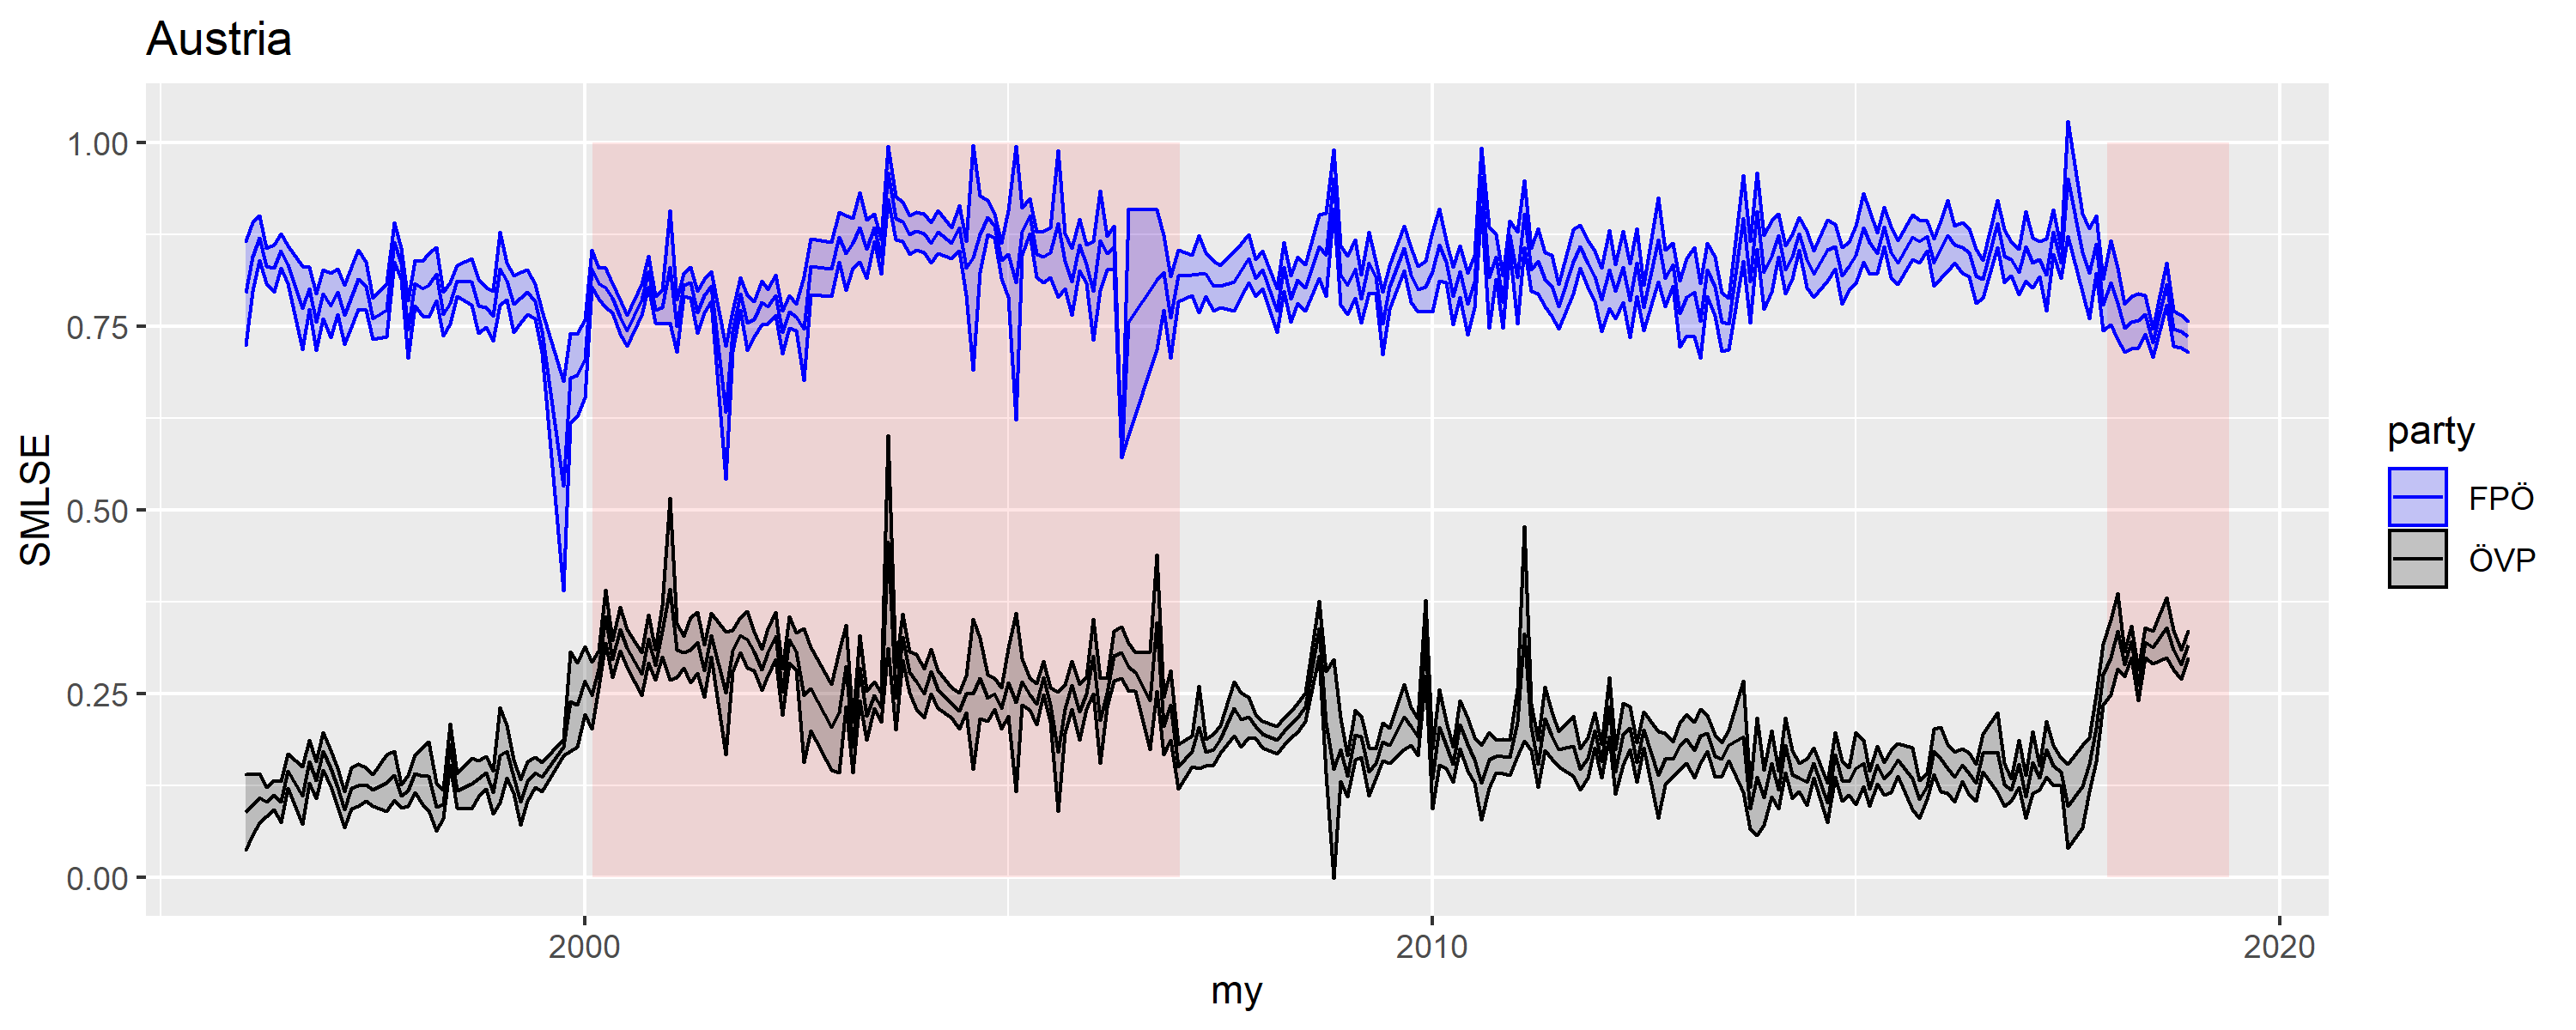
\includegraphics[width=\linewidth]{AT/vis/AT_fpvp_paper.png}
\end{minipage}
\hfill
\begin{minipage}{\textwidth}
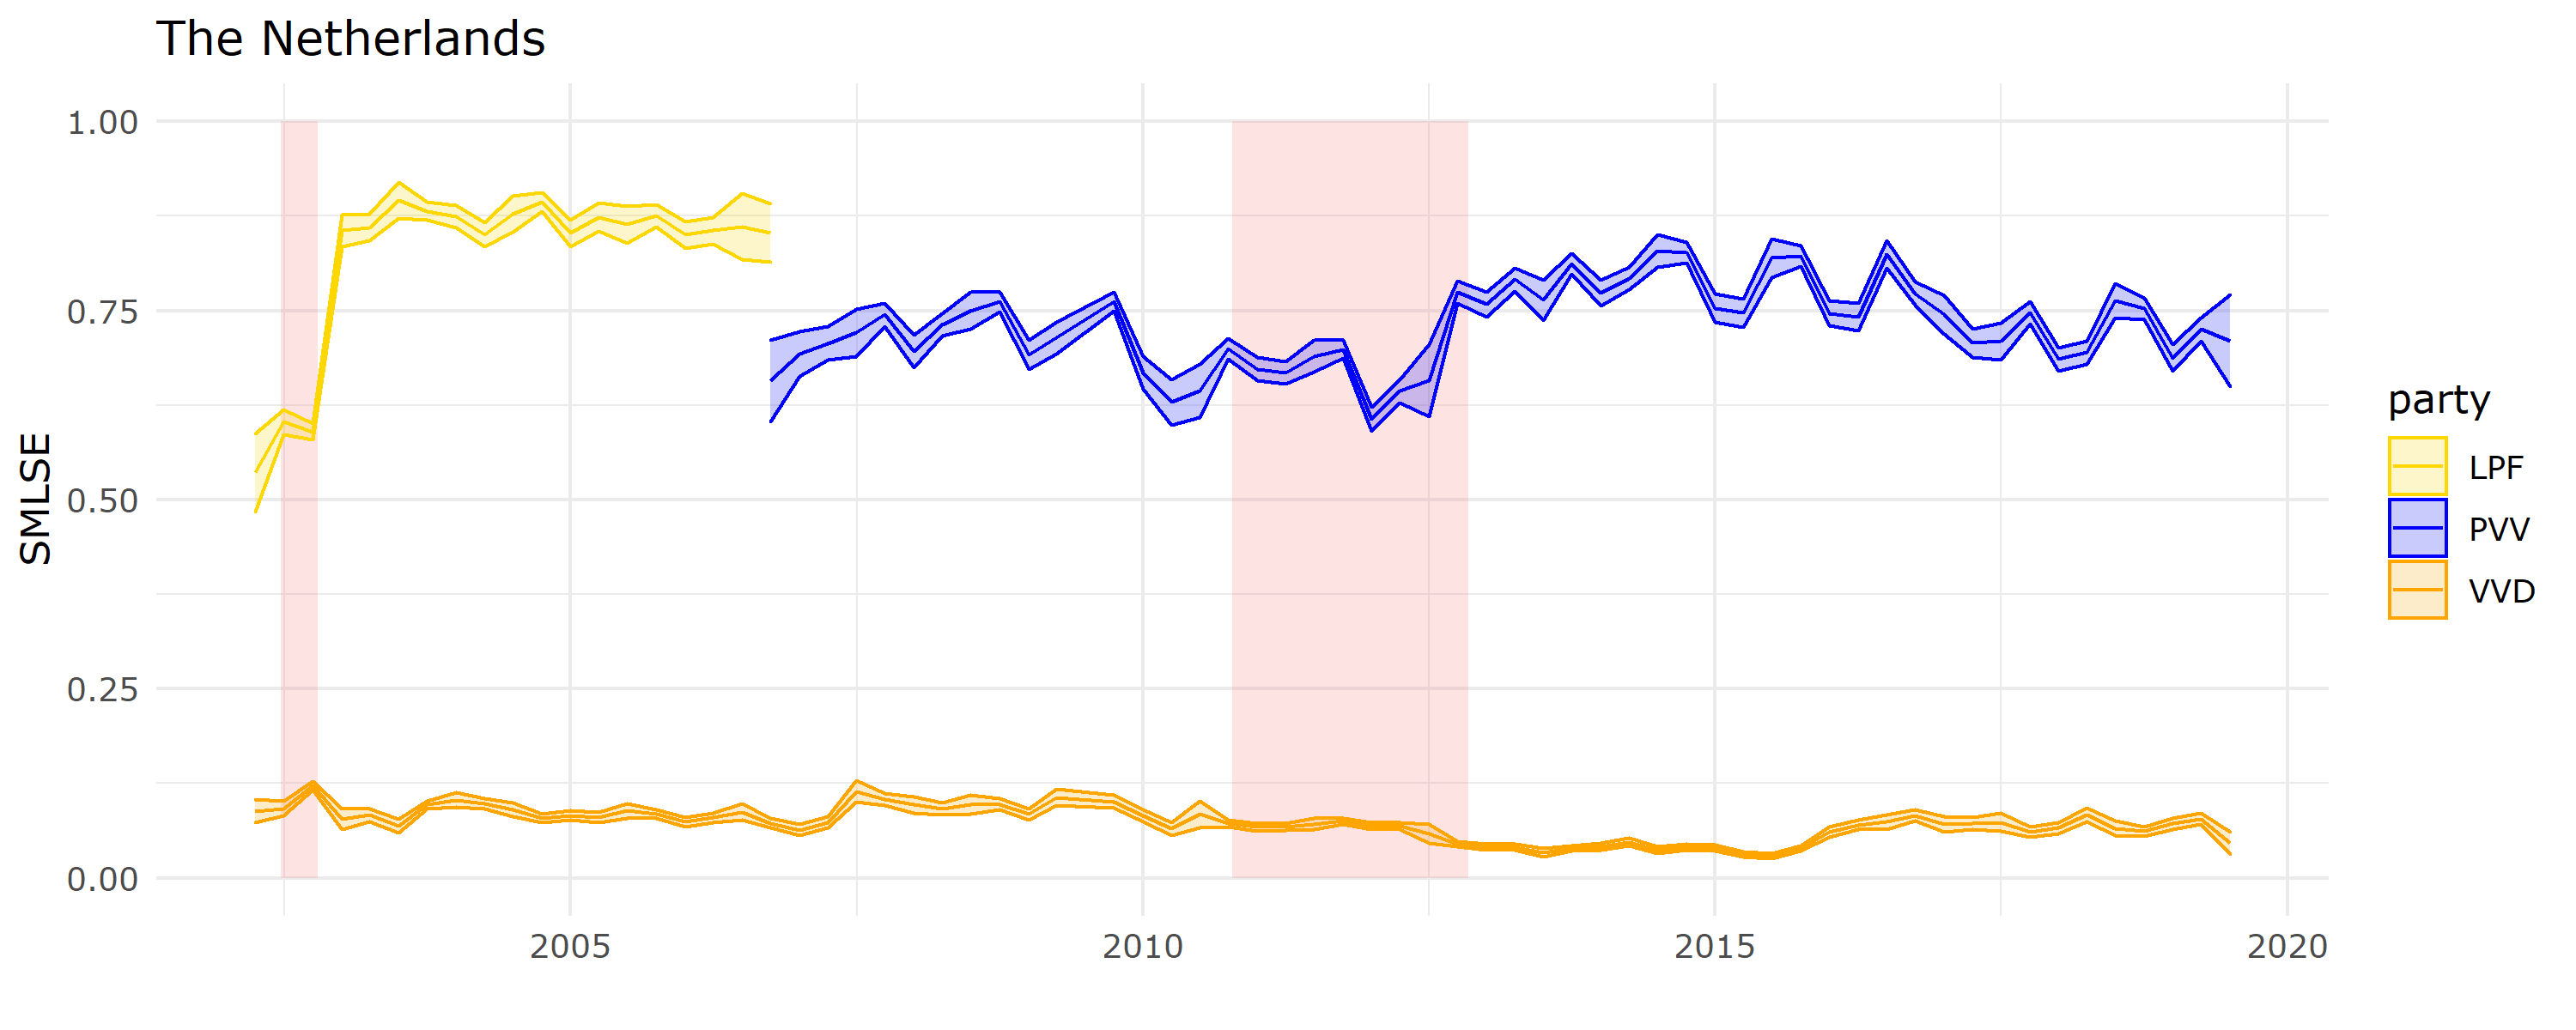
\includegraphics[width=\linewidth]{NL/vis/nl_vvd_rr_paper.png}
\end{minipage}
\caption{Monthly average similarity to radical-right parties for centre-right and radical-right parties in Austria and the Netherlands with 95\% confidence intervals. Red shaded areas indicate coalition governments and cooperation in minority governments.}
\label{fig:govs}
\end{figure}

The top row in figure \ref{fig:govs} shows the monthly SMLSEs for ÖVP and FPÖ across time. The BZÖ was excluded for ease of interpretation\footnote{See figure \ref{fig:bzoe} in appendix B1 for a graph including the BZÖ.}, but the estimate contains the classifier estimate for similarity to either radical-right party, i.e. the likelihood that the speaker belongs to \textit{either} BZÖ or FPÖ\footnote{See appendix B2, figure \ref{fig:fponly} for estimates of 'FPÖ-ness' only.}. The red shaded areas are the periods in which the ÖVP governed together with either of the two parties. A first observation is that the parties seem to move closer together when governing. This is confirmed by t-tests, which show that the distance between the two parties is significantly reduced (t=-10.2, p$<$0.001). Interestingly, this seems to be driven largely by the ÖVP (t=12.4, p$<$0.001), while the FPÖ is only slightly less distinctive in government (t=-1.68, p<0.1). \par

More interesting patterns are visible. Preceding the formations in 2000 and 2018, the conservatives became more similar to the radical-right, possibly signalling interest in coalition formation with the party. In 2003 however, the party becomes less similar for a short period\footnote{This is more pronounced in the FPÖ-only estimate excluding the BZÖ, see figure \ref{fig:fponly} appendix B2.} - they were in coalition talks with the Greens at the time and either expected heavy concessions from the FPÖ (which was already asking to govern again), or wanted to change course (\cite{Luther2010}: 91). The FPÖ, on the other hand, became less distinctive before the first formation in 2000 - possibly related to Haider's efforts to calm worries about the parties' Nazi past (ibid: 84); but more distinctive before the formation in 2018, where the ÖVP challenged the FPÖ's issue ownership on immigration, while the FPÖ underlined its 'orginalness' (\cite{Bodlos2018}). It is also visible how the FPÖ became more distinctive after the 'Knittelfeld crisis' in September 2002, where party members challenged their leadership in open opposition to their course (\cite{Luther2002}). \par

The Netherlands saw only one formal coalition government between radical-right and centre-right, but a additional minority government supported by the radical-right PVV. In 2002 the \textit{Lijst Pim Fortuyn} (LPF) brought unprecedented volatility and polarisation into Dutch politics (\cite{Bischof2019a, VanderBrug2003}). Only formed about three months preceding the election, the party gained wide attraction due to its charismatic leader, a strong media presence and its distinctive anti-immigration stance (\cite{Koopmans2009}). On election day, nine days after the party leader Pim Fortuyn was assassinated, the party came in second with 17\% of the vote and formed a coalition with the christian-democrat CDA and the centre-right VVD. Having lost its founding father and as a result of its rapid success, the party was unprepared for government and was turmoiled by internal power struggles. This peaked when two LPF ministers stopped talking to each other. As a result, CDA and VVD broke the coalition only 87 days after its formation (\cite{Heinisch2003, Lucardie2007LPF}). I expect especially the LPF to become less distinctive here, as the party members decide to enter a coalition government. Similarly, CDA and VVD should become more alike the LPF in government.\par

The co-operation of VVD, CDA and PVV in 2010 did not result in a formal majority coalition (partly due to internal conflicts in the CDA regarding a coalition with the radical-right PVV), but a 'supported minority government'. This was the first minority government formed in the Netherlands since 1922. VVD and CDA staffed the cabinet, while the PVV only promised support on major issues. As this support was settled in a formal agreement, this government became basically a 'majority government in disguise' (\cite{Strom1990, VanHolsteyn2011}). In fact, the government cooperated very little with the opposition even compared to full majority governments - this is likely an outcome of the sorting of parties into a right-wing government and a left-wing opposition but underlines the similarity of this government to classic majority coalitions (\cite{Otjes2014}). As a result, I expect an increased similarity of the coalition partners, slightly less than in a majority coalition. \par

The lower row of figure \ref{fig:govs} shows the monthly average SMLSE in the Netherlands for PVV, LPF, and VVD\footnote{CDA and FvD were excluded to maintain readability. The full plot can be found in figure \ref{fig:cda}, appendix C.}. The LPF is rather similar to all other parties when in government, obtaining a distinctiveness estimate of only around 60\%\footnote{This value can be interpreted as the confidence with which the classifier identifies LPF speeches as such.} throughout the time governing. Once the party leaves the government, the party becomes very distinctive again. For the VVD, we can observe a slightly increased score when governing with the LPF. For the supported minority government in 2010, things are far less clear. The VVD's estimate seems to remain rather stable, with possibly a slight \textit{decrease}, while the PVV becomes much less distinctive just \textit{before} signing the support agreement. Afterwards, the PVV stays somewhat indistinctive throughout the time supporting the government at around 60\% - 70\%. After the time in government, the party's communication becomes more distinctive again.\par

T-tests confirm these observations. The LPF does show a significantly decreased distinctiveness in government (t=-6.15, p$<$0.01), as does the PVV (t=-5.36, p$<$0.001). The VVD only shows slightly increased similarity to the respective radical-right party when governing with the LPF (t=3.21, p$<$0.1), but when supported by the PVV, this effect becomes virtually zero (t=0.6, p=0.55). The CDA is assigned similar SMLSEs, though more clearly reacting to the LPF (t=7.1, p$<$0.01), but neither to the PVV (t=0.96, p=0.34). Overall, the VVD is not significantly affected by governing with a radical-right party (t = 1.64, p$>$0.1), while the CDA is significantly changing its rhetoric (t=2.01, p$<$0.05).\par

Additionally, throughout the time in government, the LPF becomes less distinctive, while the VVD seems to become more similar. This is in line with an ideological shift in the VVD's manifesto, which took up a more anti-immigrant position (\cite{Pennings2003}), while the LPF dropped some of it's populist rhetoric (\cite{Lucardie2007LPF}). For the PVV, a shift towards the centre is visible before the formation of the minority support government - possibly signalling willingness to govern, similar to Haider's FPÖ preceding the Austrian elections in 2000.\par

The findings are in line with my expectations: governing parties are more similar to each other - the estimates display construct validity. Interesting variation can be observed across countries and different government formations. While it is mainly the centre-right which accommodates the radical-right in Austria, it is usually the radical-right which becomes more similar in the Netherlands, even when only supporting a minority government. This might have to do with the differing coalition logic in the two countries. The ÖVP held the ideological middle-ground of the three major parties and was able to choose with whom to form a coalition - both in 2000 and 2017, the party decided against a continuation of the coalition with the social democrats. In the Netherlands, coalitions often include many parties, which gives those in charge of forming a government many options. The moderation on behalf of the PVV may have been necessitated by the resistance from parts of the CDA against the formation of a coalition with the PVV. Interesting is also that radical-right parties often moderated before coalition formations, possibly signalling willingness to govern. Only the FPÖ reacted to the ÖVP's accommodation in 2017 with further distinction. These observations indicate possible starting points for future research with this method and underline the richness of the data.\par



\subsection{Construct validity II: speaker estimates}

Beyond parties, the similarity or distinctiveness of particular speakers can also be of interest. I use two cases from Germany and the Netherlands to further validate the method's precision. In both cases, I have strong expectations about the placement of individual speakers. In Germany, six members of the AfD have since left the party, mainly due to the increasing strength of the far-right faction within the radical-right party (\cite{Steffen2020AfD}). Two of these members, one of whom was former party leader Frauke Petry left within the first ten days following the election (\cite{LSE2018AfD}). As they were members of the party themselves, these members should obtain higher similarity scores than members of other parties\footnote{Note that the data contains no speeches by these two independent members preceding their exit, excluding a longitudinal analysis comparing their similarity before and after exit.}. Similarly, four members of the AfD who left the party later (outside of the observed time-frame) should obtain lower similarity scores, compared to loyal members of the AfD. \par

\begin{sidewaysfigure}
    \centering
    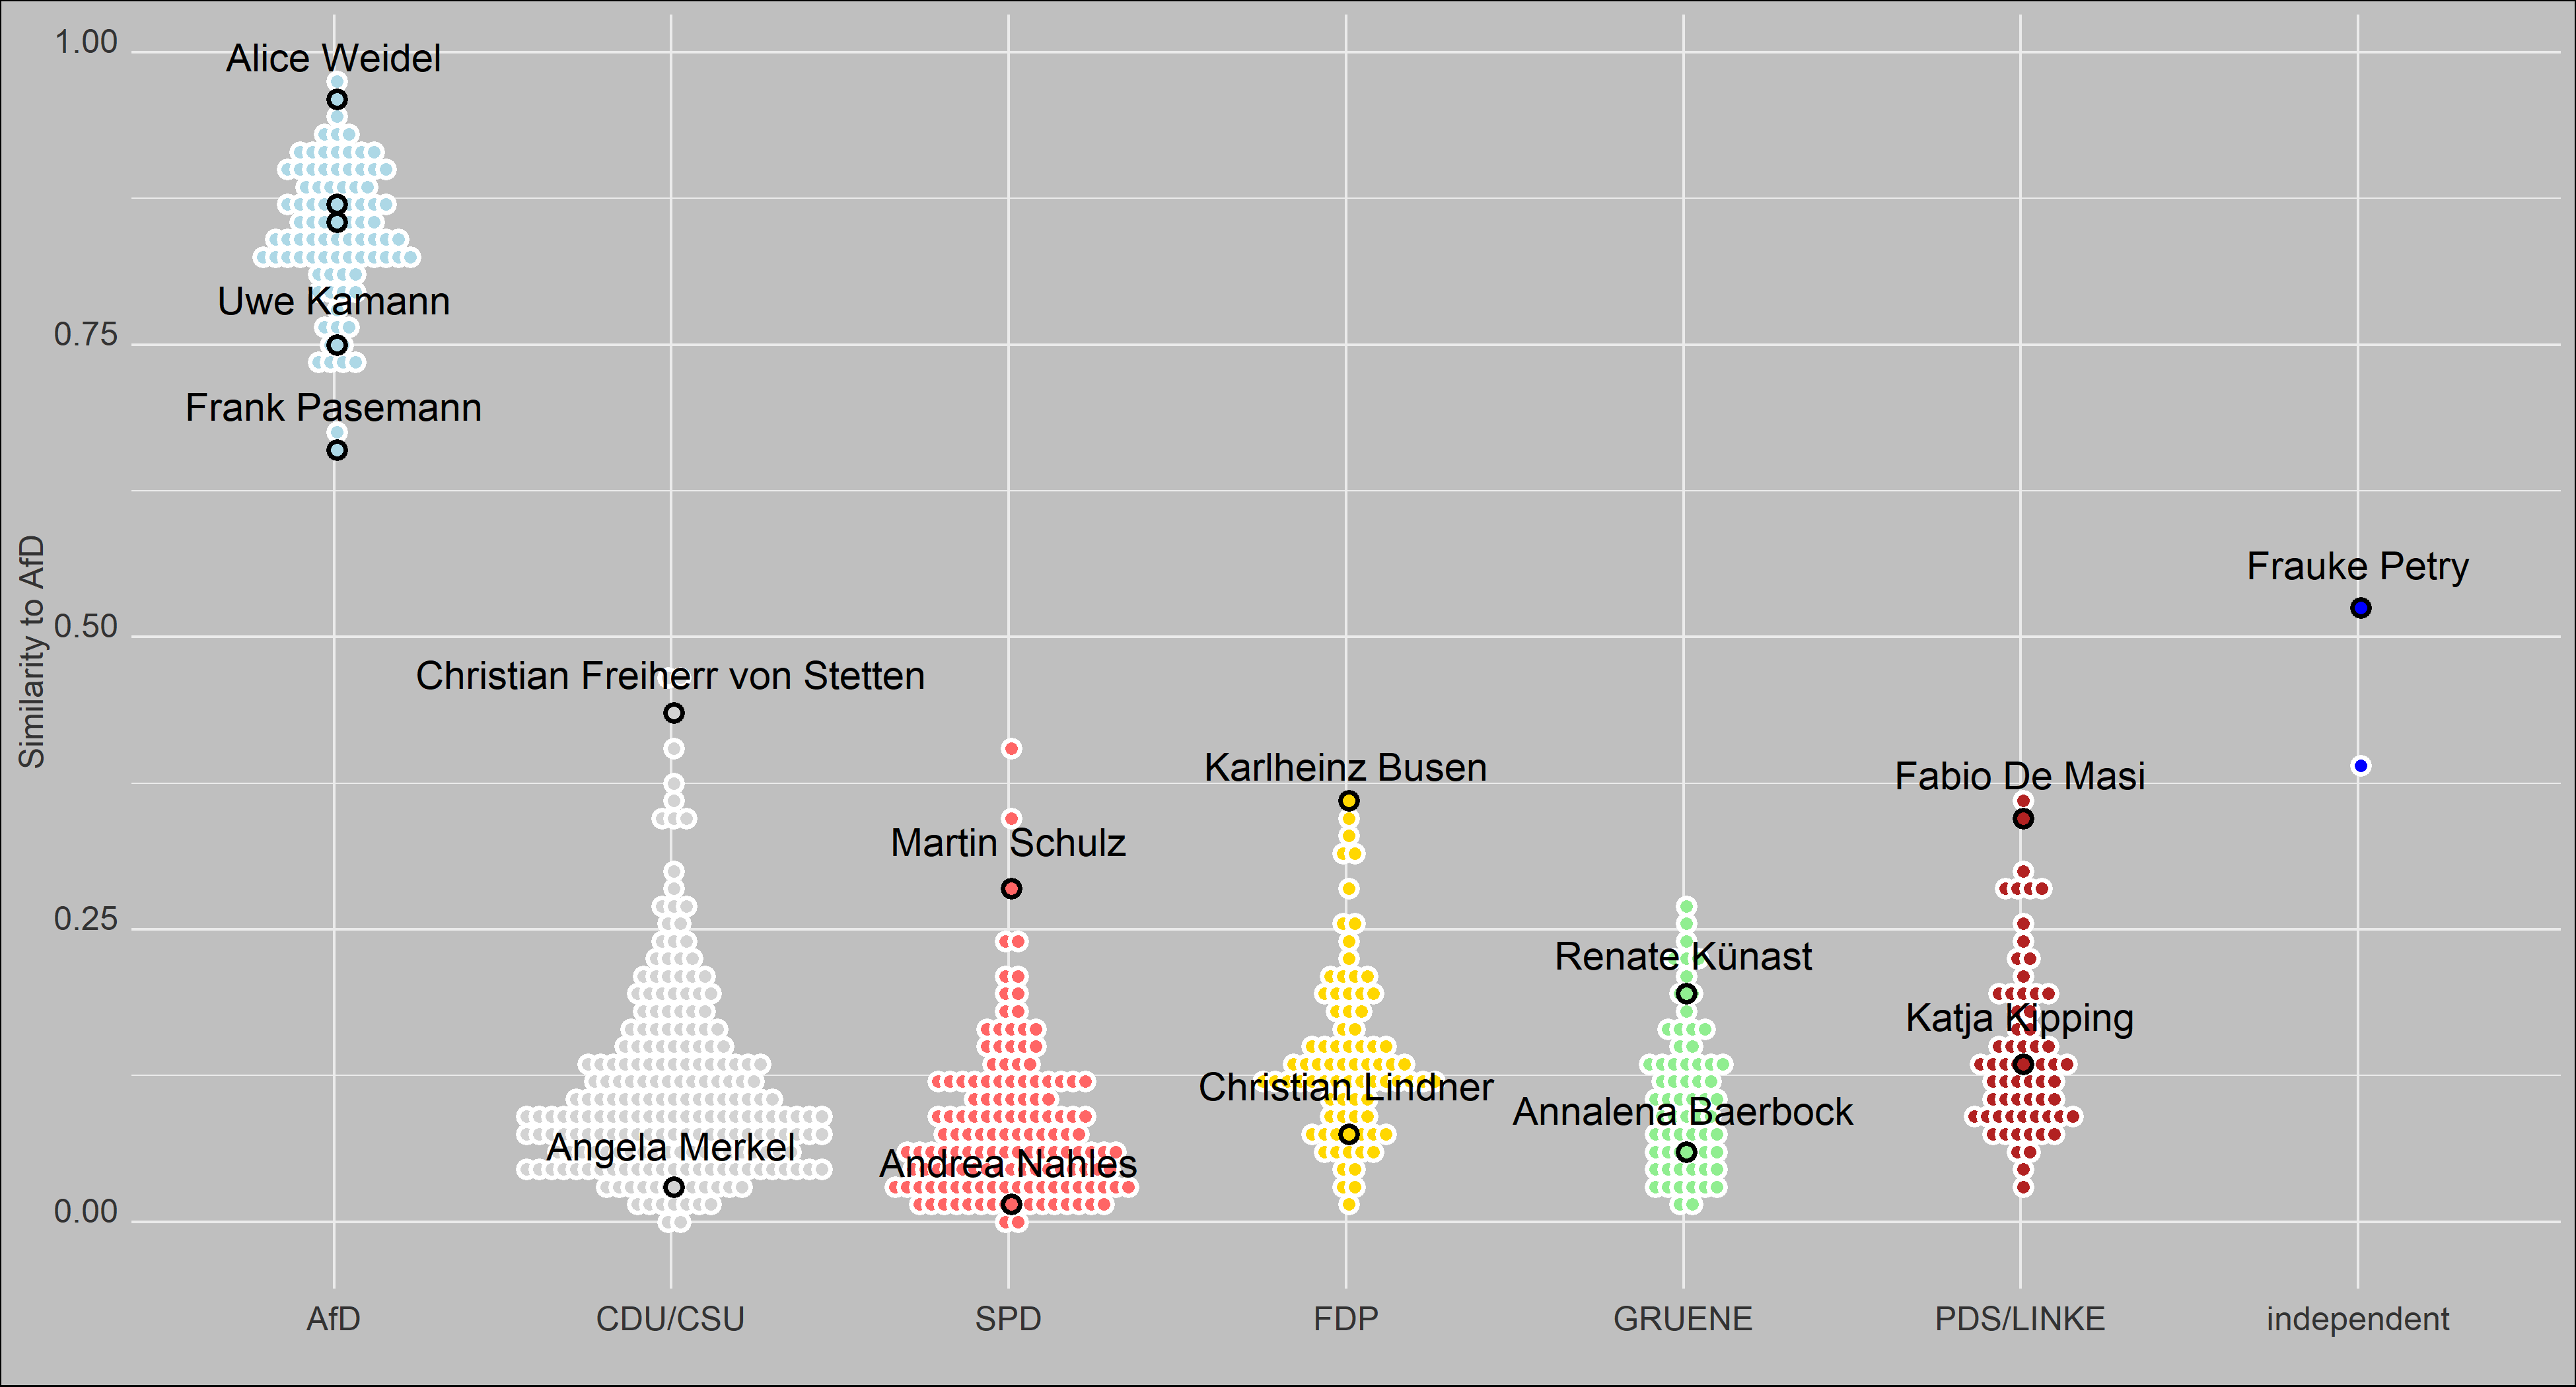
\includegraphics[width=19cm]{DE/vis/DE_speakers.png}
    \caption{SMLSEs for speakers of the current German Bundestag.}
    \label{fig:speakers}
\end{sidewaysfigure}

Figure \ref{fig:speakers} shows the mean estimate for each speaker in the current Bundestag. Each speaker is represented by a dot. The dot's position on the vertical axis indicates the speaker's similarity to the AfD, according to the SMLSE, while its color and horizontal position indicate the speaker's party affiliation. The classifier assigns a probability greater than 0.5 for all AfD-members and a probability smaller than 0.5 to all speakers from established parties. In line with my expectation, the now independent former members of the AfD obtain rather high values (Frauke Petry: 52.6\%, Mario Mieruch: 39.3\%) and are located in between the AfD and the other parties. The mean estimate for all speeches by these two speakers is distinctive from all other parties. Despite being labelled not to be part of the AfD in the training data, the classifier correctly locates them in proximity of the AfD. \par

Uwe Kamann would leave the AfD five days after the observed period ends, on December 17th, 2018. His estimate is relatively low compared to his party, however several members obtain lower estimates. Lars Herrmann and Verena Hartmann, two other members that left the AfD, followed in winter 2019/2020, about one year after the data ends. In the data observed, the classifier still places them well inside their party (see two highlighted, unlabelled dots within the AfD). For these ex-members of the AfD, the expectations are not confirmed. It might be the case that they still move to the fringes of their party in the following year. The estimates for Frank Pasemann, the sixth member in the data to leave the party (and the only one to do so involuntarily), exemplify well how SMLSEs work. Pasemann was expelled from the AfD in August 2020\footnote{\href{https://www.mdr.de/sachsen-anhalt/landespolitik/afd-politiker-pasemann-aus-partei-ausgeschlossen-100.html}{https://www.mdr.de/sachsen-anhalt/landespolitik/afd-politiker-pasemann-aus-partei-ausgeschlossen-100.html}}, most likely as a result of anti-semitic statements and his proximity to members of neonazi- and radical-right associations\footnote{\href{https://www.mdr.de/investigativ/afd-pasemann-ausschluss-extrem-rechte-100.html}{https://www.mdr.de/investigativ/afd-pasemann-ausschluss-extrem-rechte-100.html}}. As the concept being measured is 'AfD-ness' (specified as the outcome category in the training data), the classifier assesses how well a speech fits into the corpus of AfD-speeches. As a result, Pasemann, who is clearly located to the right of his party, obtains lower estimates than other members of his party.\par

Beyond these specific members, all parties show considerable variation. The overall distribution of the two governing mainstream parties is skewed towards the lower end of the scale, with only few members in the tails with higher probabilities. This tail is more pronounced for the CDU/CSU. Among the conservatives, the measure seems to have an ideological component: those with a high probability of being members of the AfD also seem to have more conservative positions. While Angela Merkel is assigned a low similarity score (2.9\%), Christian Freiherr von Stetten (43.2\%) and other more conservative members of the party are placed more closely to the AfD. Stetten is not very present in the media, he was a vocal advocate of a conservative turn of his party under the leadership of Friedrich Merz (\cite{Weinzierler2019}), and has been affiliated with the conservative WerteUnion, which works towards a right-wing turn in German politics\footnote{He is quoted as a supporter (including a picture of his face) on the movements website: \url{https://werteunion.net/}}. Within the SPD, it is interesting that delegates from former industry regions in North Rhine-Westphalia and Eastern Germany like Dirk Vöpel (40.8\%), Detlef Mueller (34.9\%), Martin Schulz (28.9\%), and Josip Juratovic (24.3\%) are assigned higher values compared to their party. However note that e.g. Martin Schultz is a fierce advocate against the radical-right\footnote{See e.g. \href{https://www.tagesspiegel.de/politik/ex-spd-chef-attackiert-afd-vorsitzenden-schulz-wuenscht-gauland-auf-den-misthaufen-in-der-deutschen-geschichte/23057642.html}{https://www.tagesspiegel.de/politik/ex-spd-chef-attackiert-afd-vorsitzenden-schulz-wuenscht-gauland-auf-den-misthaufen-in-der-deutschen-geschichte/23057642.html}}. This might indicate rhetorical rather than ideological similarity - the classifier does not distinguish.\par

The estimates for the other opposition parties are somewhat more spread out than the two governing parties, but with similar tails towards the top. Within the FDP, Karlheinz Busen gets assigned the highest estimate of his party (35.3\%). His political positions revolve around agricultural matters \footnote{\url{https://karlheinz-busen.de/}}, which is an issue that the AfD is increasingly trying to mobilise on \footnote{\url{https://www.sueddeutsche.de/politik/afd-bauern-landwirte-1.4764413}}.  Among the Linke, several members obtain rather high estimates, most prominently Fabio de Masi (34.6\%), a politician with a strong focus on EU-policy, where the party holds a Eurosceptic position\footnote{\url{https://www.fabio-de-masi.de/de/topic/15.eurokrise.html}} (as does the AfD; \cite{ThePopulist2019}).\par


In the Netherlands, the rise of the LPF and the subsequent politicisation of immigration forced other parties to react to the issue (\cite{DeVries2012c, Pennings2003}). This proved a wedge issue for the VVD, pitting the social-liberal faction around state secretaries Mark Rutte and Melanie Schultz against party members demanding a shift to the right, most famously Geert Wilders (\cite{VandeWardt2014, Vossen2011}). After being described as a likely candidate for party leadership of the VVD in the early 2000s (\cite{Vossen2011}, 182), Wilders developed an increasingly extreme anti-islamism from 2003 onwards (\cite{Vossen2010}, 26). This alienated him from the social-liberal wing of the VVD and the party's leadership, especially parliamentary group leader van Aartsen. In 2004, Wilders published a position paper together with his fellow VVD MP Gert-Jan Oplaat calling for a right-wing turn in the VVD. It was speculated whether Wilders would join the LPF, which held similar anti-muslim and anti-immigration positions (\cite{Parool2004Wilders, Handelsblad2008Wilders}). After several calls by the leadership to follow the party line, he left the VVD to form the radical-right PVV, while the VVD took a more centrist course (\cite{Vossen2010, Vossen2011}). \par

 As Wilders develops more anti-muslim positions, I expect him to become more similar to the LPF in the time preceding his exit, compared to other members of the VVD. This should especially be the case when compared to proponents of the social-liberal course of the VVD. Immigration-critical members of the VVD like Gert-Jan Oplaat (who co-authored the position paper with Wilders), Ayaan Hirsi Ali (who co-authored an op-ed with Wilders calling for a 'liberal Jihad'; \cite{Vossen2011}, 183) and Rita Verdonk (who later formed her own populist party \textit{Trots}) should be placed in proximity of Wilders. \par


\begin{figure}
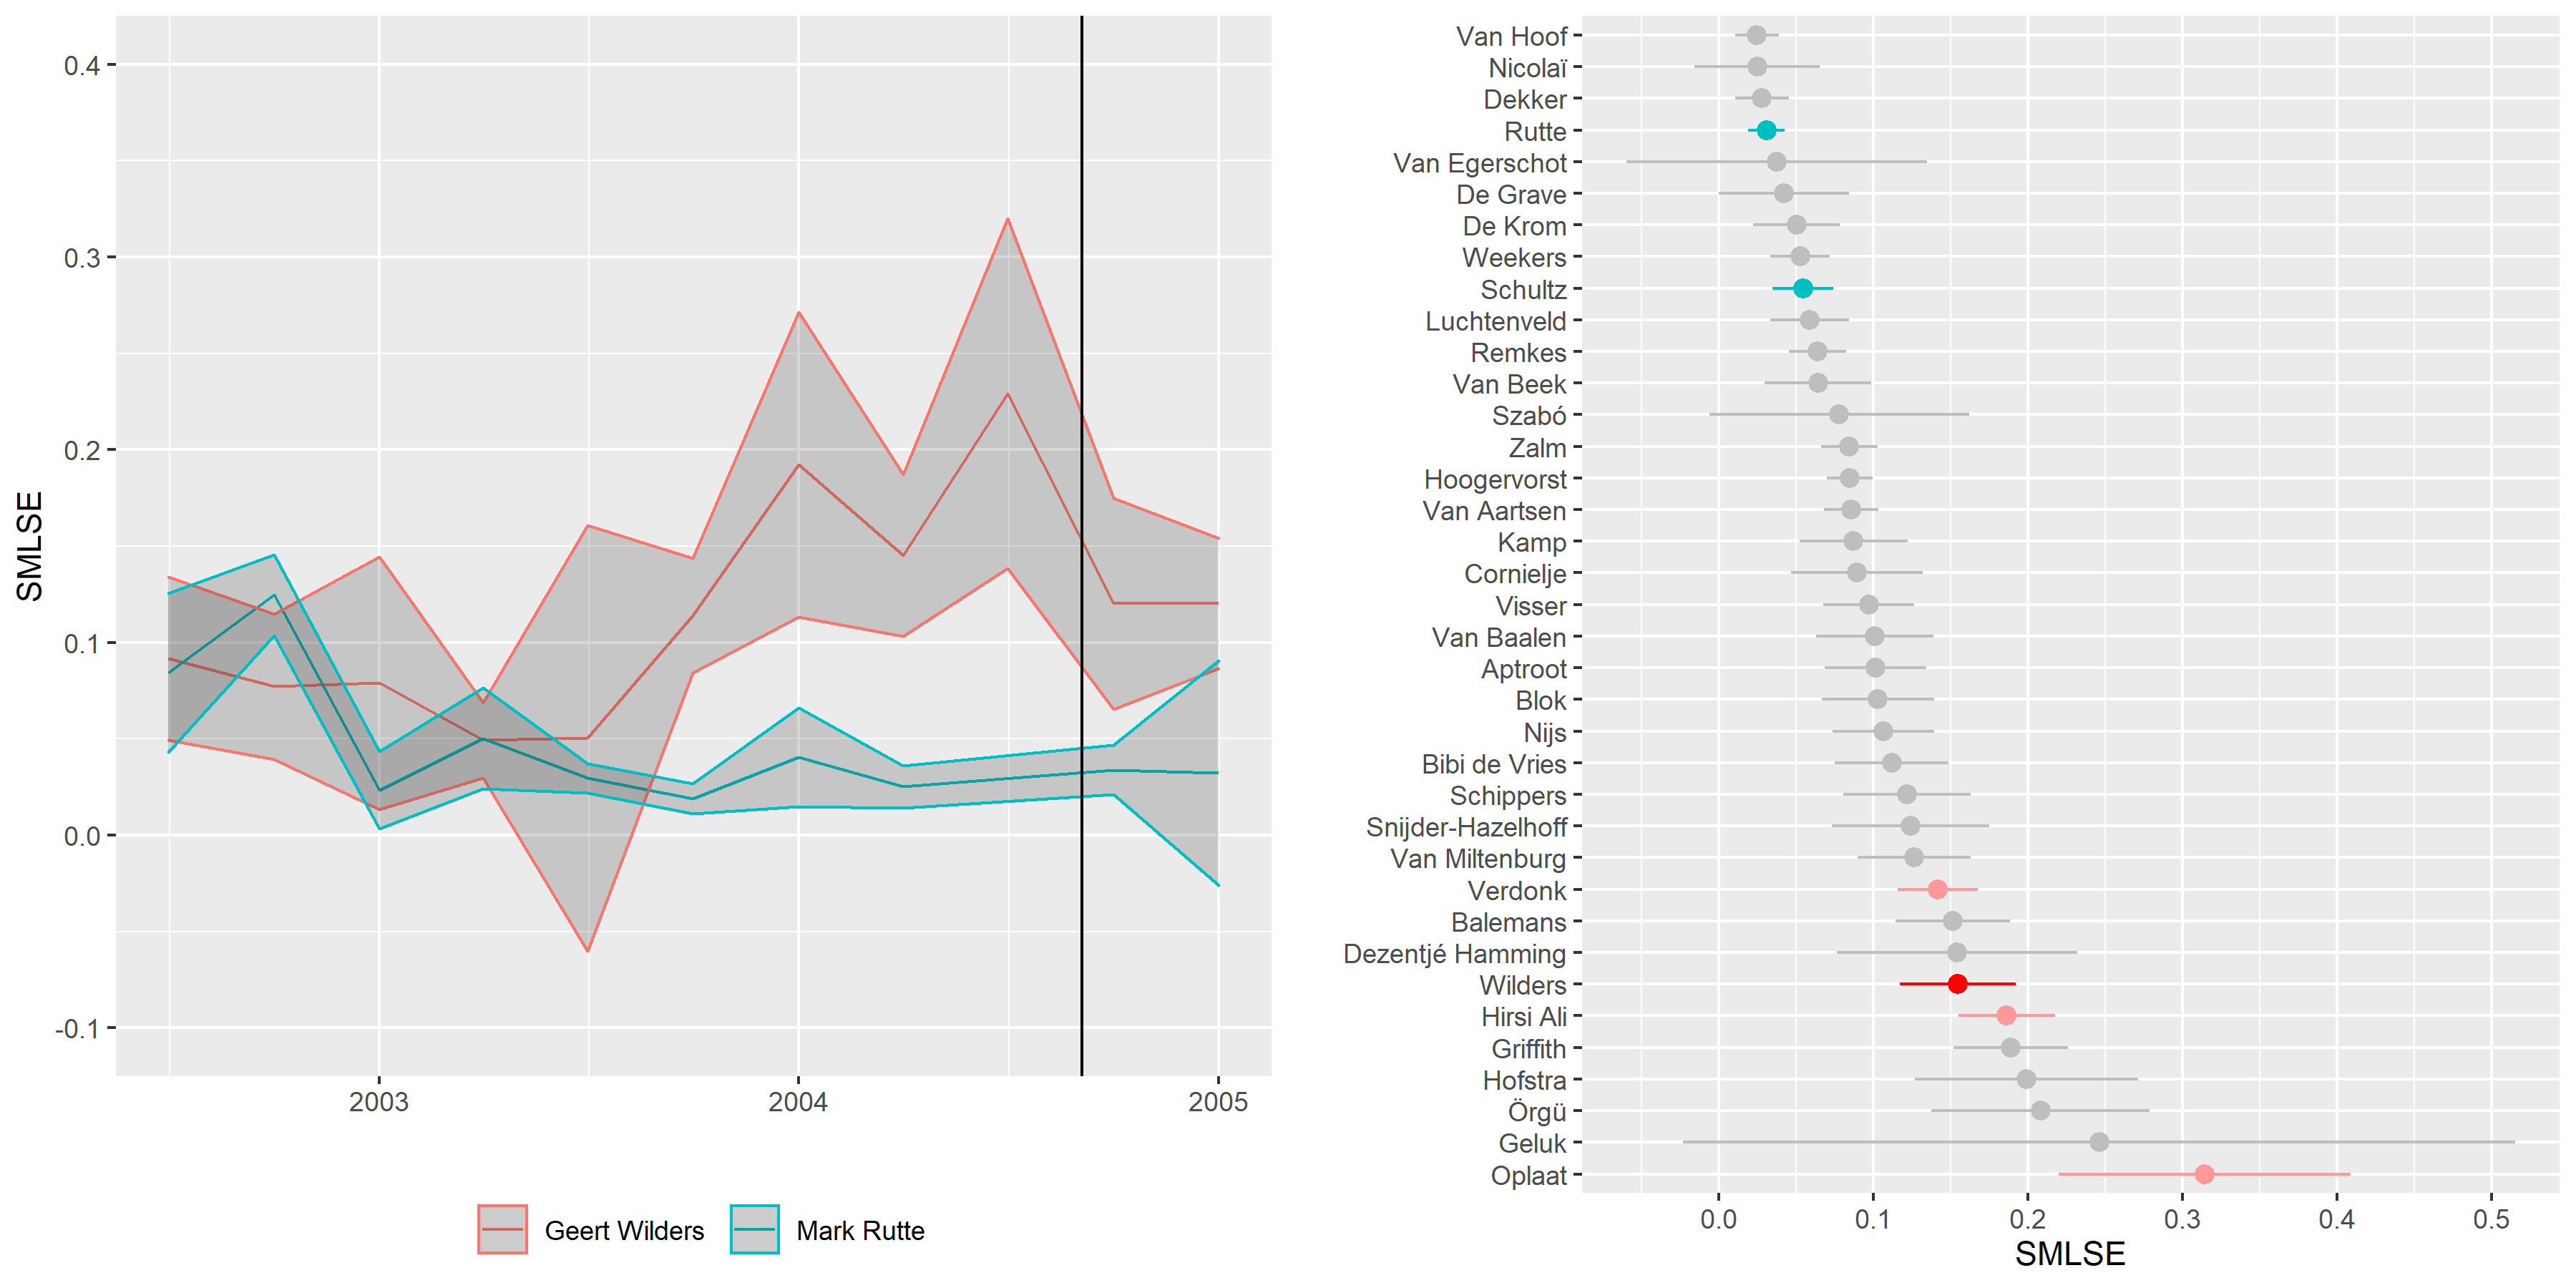
\includegraphics[width=\linewidth]{NL/vis/Wilders_both.png}
\caption{\textbf{Left}: quarterly SMLSE estimates for Geert Wilders and Mark Rutte in 2004. The vertical line indicates the date Wilders' left the party. \textbf{Right}: Placement of Wilders (red), compared to social-liberal (turquoise) and right-wing members (light-red) within the VVD in 2004, preceding Wilders' exit. Both graphs show the estimates with 95\% confidence intervals.}
\label{fig:wilders}
\end{figure}

The left graph in figure \ref{fig:wilders} shows the quarterly mean SMLSE of Geert Wilders and (at the time) more socially-liberal oriented Mark Rutte, from the first entry of the LPF until Wilders' exit. It is visible that in 2002 and 2003, both estimates overlap at low levels. The classifier gives both speakers a 0-10\% chance to belong to the LPF. In line with my expectation, Wilders' estimate moves upwards from mid-2003, indicating higher similarity to the radical-right LPF, until mid-2004 (the last estimate before Wilders left the party), when the classifier assigns a likelihood over 20\% that this speaker might belong to the LPF. This is especially extreme compared to the significantly distinctive estimate for Rutte at below 5\%. It seems that after the election, an issue sorting takes place, as Wilders embraces the LPF's position, while Rutte further distances himself (\cite{Carmines1986}). After his exit, Wilders' language changes again, becoming less alike the LPF.\par

Based on the scores alone, it is unclear what drives the increased similarity of Wilders' language to the LPF. The expectation is that the distinction should revolve around Islam and immigration, the major issue that Wilders' party mobilized on later (\cite{VanHolsteyn2011}). Disagreement on these issues was also reflected in the support agreement between VVD, CDA and PVV in 2010 (\cite{Otjes2014}, 350). I calculate each word's influence on Wilder's SMLSE  by multiplying the model coefficient with the (tfidf-weighted) word count from all his speeches between the second CDA-VVD-LPF government formation until his exit from the VVD in 2004. The 30 words with the strongest positive influence\footnote{See table \ref{tab:wilders} in appendix D.} contain several terms related to Islam ('imam', 'mosques'), security ('AIVD'\footnote{AIVD is the Dutch intelligence service.}, 'Defense'), terrorism ('terrorists'), and muslim countries ('Algeria', 'Saudi', 'Arabia'), as well as 'Europe'. It seems that Wilders' increased similarity in this period is indeed related to his increased attention to Islam.\par

The right side of figure \ref{fig:wilders} shows Wilders' placement compared to other VVD members. In general, Wilders is placed relatively similar to the LPF, obtaining the 7th-highest estimate (20\%) of the 37 members covered by the data. Likewise, other members opposed to Islam and immigration (Hirsi Ali, Oplaat, Verdonk) obtain similarly high estimates, while the proponents of a social-liberal course (Rutte, Schultz) are assigned relatively low estimates.\par

Although far more detailed, the speaker estimates are in line with expectations, underlining the precision of the method. The former members of the AfD were placed in between the AfD and all other parties. The member leaving the party shortly after the observed period is placed relatively low within the party. Surprisingly, the two members who would leave one year later are placed relatively central within the party - at the time, there was no indication that they might leave. Assessing the VVD in 2004, the estimates correctly place social-liberal and more right-wing members within the party. Even more impressive, Geert Wilders' divergence from the VVD from 2003 onwards is significant in the estimates.\par 



\section{Comparative Performance}
The SMLSE estimates conform to expectations in all described cases. Nevertheless, existing methods could be used to estimate rhetorical similarities. This section compares SMLSEs for the current German legislature to cosine similarity and wordfish estimates. Cosine similarity is a relatively simple measure, which has seen political science applications (see e.g. \cite{Similarity2007a, Hager2020}). It takes the cosine of the angle of two document vectors to assess their similarity. It equals one when the two compared documents are identical in their relative word usage and zero when the documents share no common words. Scaling methods like wordscore (\cite{Laver2003}) and wordfish (\cite{Slapin2008}) have become popular to estimate differences in party communication, mainly to place texts on an ideological scale. \par

\subsection{Cosine similarity}

Cosine similarity is calculated for each document, comparing it to all AfD-authored speeches, then taking the mean similarity score. This results in very low overall similarity scores, ranging between 0.04 and 0.05. Figure \ref{fig:comp} shows the mean speech estimates for SMLSE, cosine similarity, and wordfish for each party in the current German legislative period. While the AfD is clearly distinguished by the SMLSE, there are only slight party differences for the cosine measure, with comparatively large confidence intervals. Cosine similarity is unable to distinguish AfD speeches, with the AfD only ranked \textit{third} in similarity to AfD speeches. This is in line with weak performance of this measure when meaning is relevant (as opposed to e.g. the detection of plagiarism, where literal similarity is relevant; \cite{Prasetya2018}).\par

The weak performance becomes more obvious once the measure is correlated with speech length: over 75\% of the variance in cosine similarity are explained by the length of the speech (Pearson's r = 0.87). It seems that the increased likelihood of a word to be included is the main driver of increased similarity here. The correlation of cosine similarity with the SMLSE is in fact weakly \textit{negative} (-0.17)\footnote{When using the logged SMLSE to normalise the distribution, this decreases to -0.36.}. AfD authorship is statistically unrelated to cosine similarity (correlation of -0.02). Calculating cosine similarity of these groups differently by first generating the average word count of AfD speeches and then calculating cosine similarity results in virtually identical results. I also calculated Jaccard\footnote{Jaccard similarity assesses the share of common words among all words used (it is unrelated to how often the words are used).} similarity with similarly weak performance.\par

\begin{figure}
    \centering
    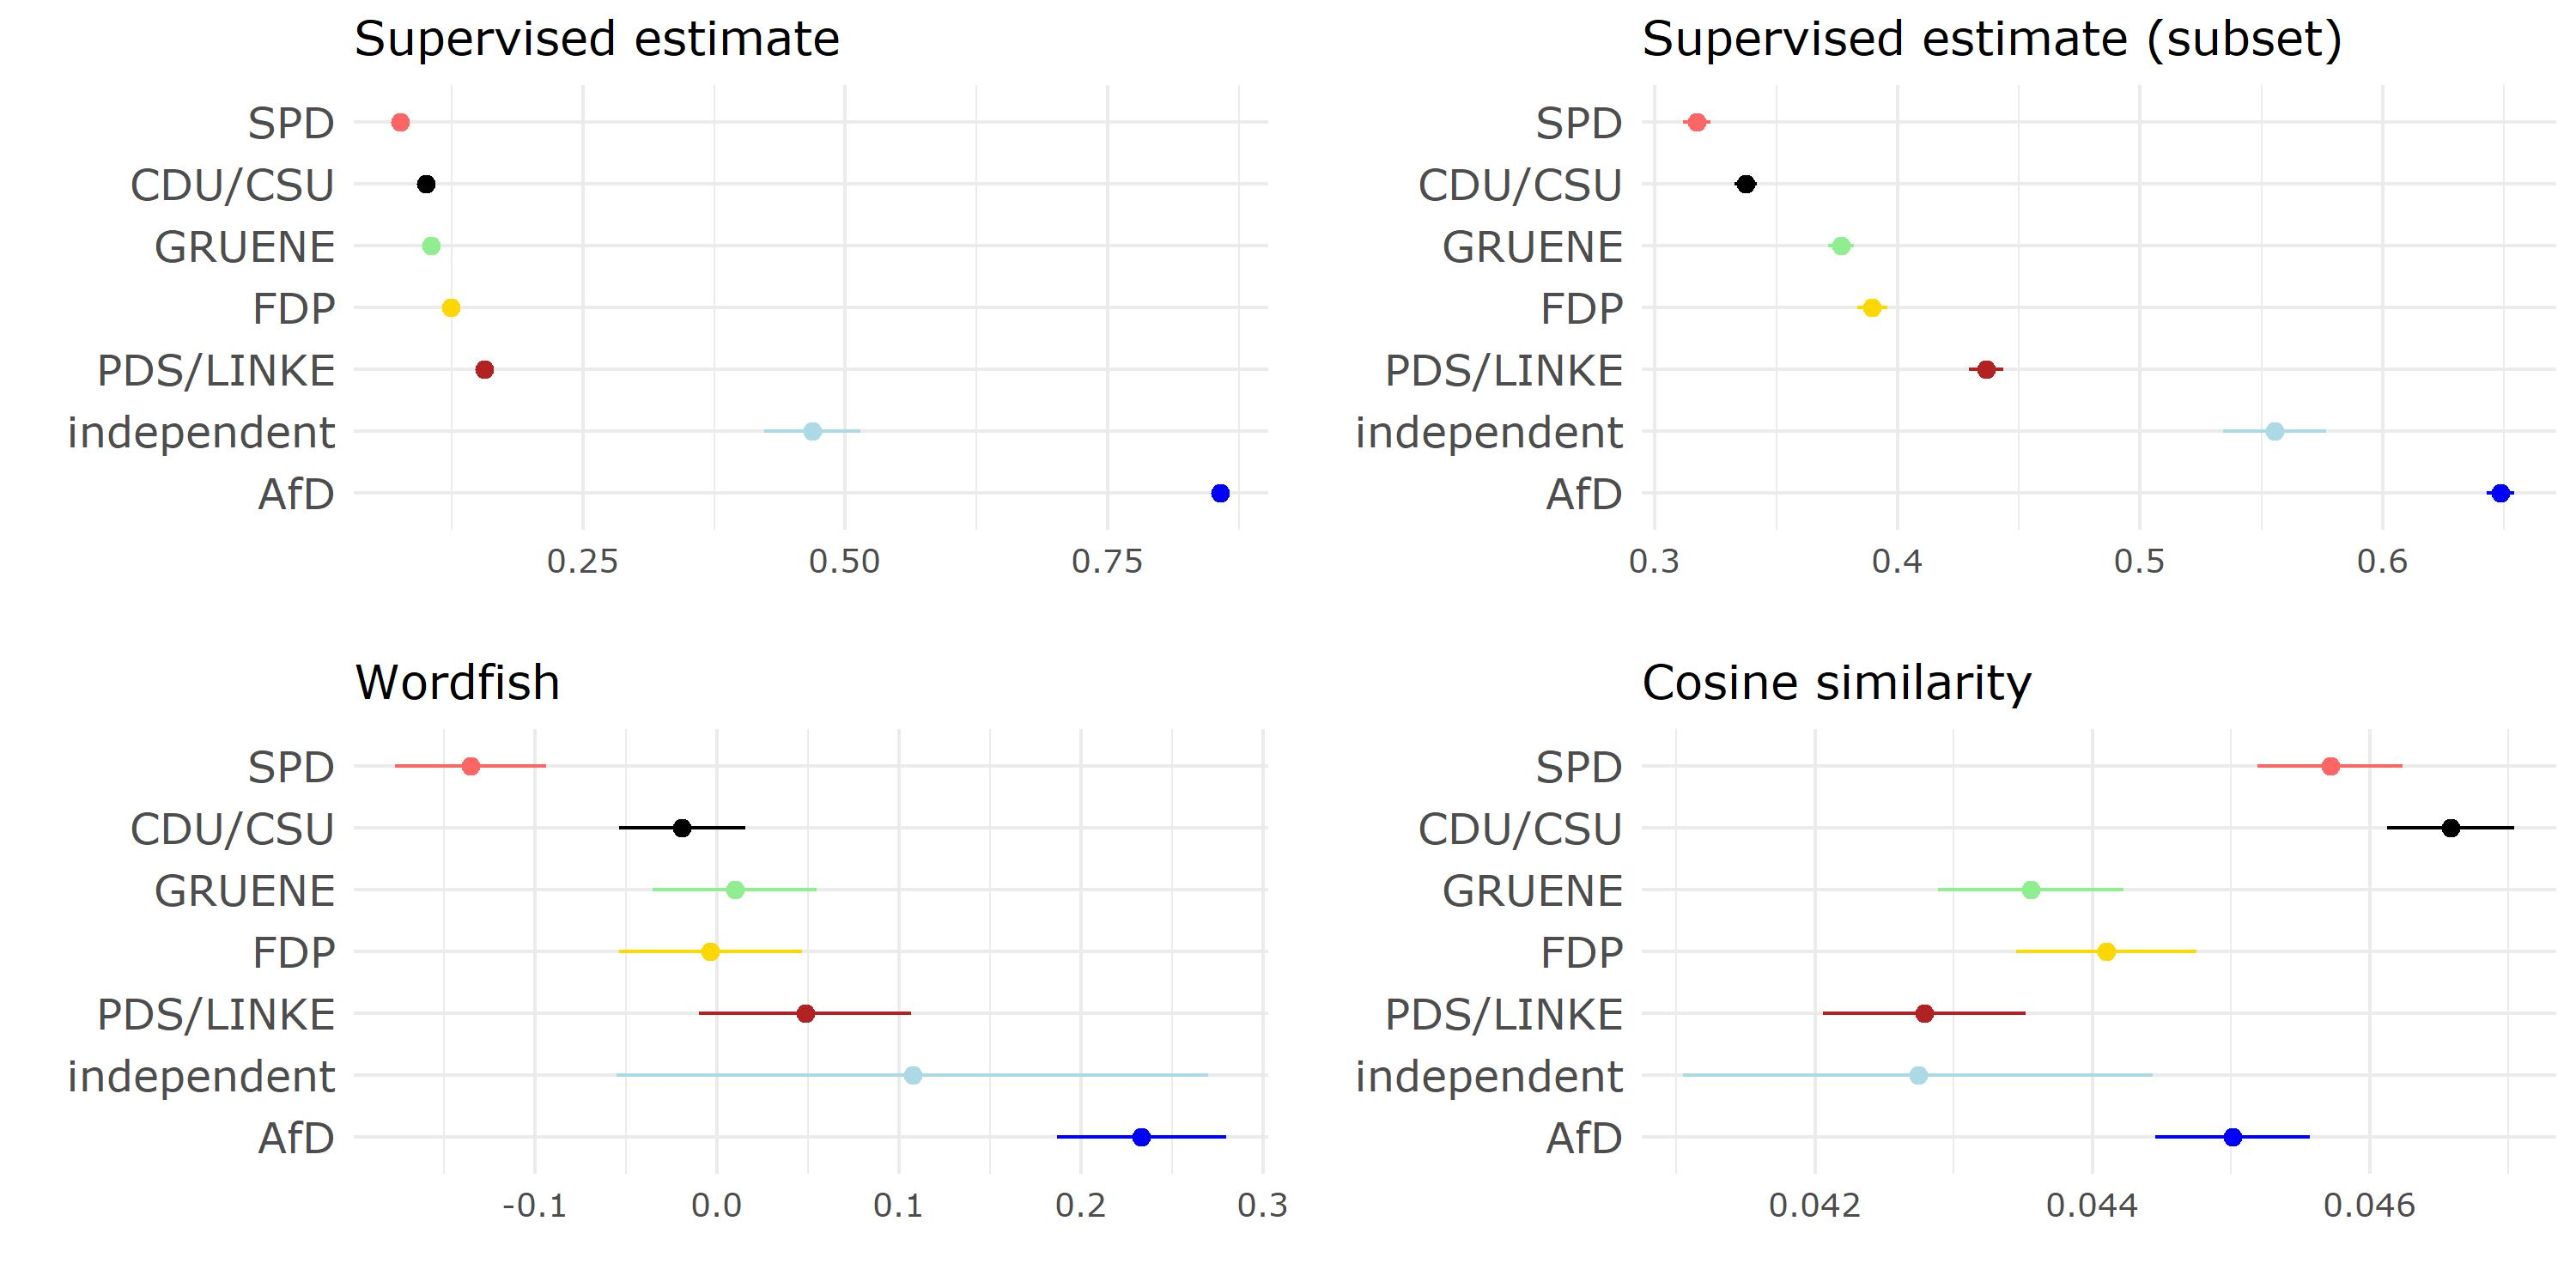
\includegraphics[width = \textwidth]{DE/vis/similarity_pts.jpg}
    \caption{Mean party estimates with 95\% confidence intervals for SMLSE, cosine similarity and wordfish estimates. Both wordfish and the restricted SMLSE model were trained on a subset of 1000 speeches, which then estimated the positions of all speeches.}
    \label{fig:comp}
\end{figure}

\subsection{Wordfish}

To assess how parties and speakers differ in word use and whether they are more or less similar, a researcher could also use scaling methods. As wordscore (\cite{Laver2003}) requires the selection and labelling of anchor documents (and hence the introduction of subjective bias), I compare the estimates from the supervised algorithm to wordfish-scores. Wordfish extracts a major underlying dimension which explains differences in word use (\cite{Slapin2008}). The SMLSE is conceptually different from wordfish estimates. Instead of estimating an underlying dimension explaining differences in word use, the SMLSE estimates a statistical model where word use explains an outcome variable (e.g. radical-right authorship) and then employs this model to assess the similarity of documents to the group of interest. \par

The last row in figure \ref{fig:comp} shows the wordfish estimates for each party. As the process was to computationally intense to be run with the full set of 11,419 German speeches\footnote{On a machine with 16GB working memory.}, I ran the scaling estimates on a sample of 1,000 speeches with at least 50 words. To make a fair comparison, the upper right graph in \ref{fig:comp} shows SMLSEs for such a subsample. A first observation is that the wordfish distributions show far more overlap than the SMLSEs\footnote{Note that the sign of the wordfish estimates has been inverted to simplify comparison.}. Other than cosine similarity measures, wordfish places the AfD very distinctly. It also correctly places the independent speakers in proximity to the AfD. Similar to the SMLSEs, the distribution does not follow a left-right pattern, but places the governing parties and especially the SPD as most distinct, the opposition parties in between and the independent speakers in proximity to the AfD. However, these estimates also show large confidence intervals and most parties' mean estimates cannot be distinguished. It is only somewhat correlated with the SMLSE (0.17, logged 0.22), although the order of the parties' mean estimates is similar - with the exception of the FDP. It seems that on the main underlying dimension structuring the differences in word use, the FDP is a little closer to the governing parties, while when the dimension of interest is the similarity to the AfD, the FDP is somewhat closer to the AfD, compared to e.g. the Greens. Furthermore, the interpretation of these scores is harder, as it does not correspond to similarity towards a group (or distinctiveness of that group). Instead, the estimates provide the placement of groups on the best fitting underlying dimension to explain the differences in word use. The interpretation of this dimension is left to the researcher. In this example, there seems to be a mixture of left-right and government-opposition dynamics\footnote{Also note that this example likely downplays the conceptual difference of wordfish and SMLSEs, as the AfD is an extreme case, where similarity seems rather correlated with the main underlying factor. This should be different if similarity towards a centrist party is investigated.}.\par

Lastly, the runtime of the estimations is also relevant, as researchers want fast analyses that save them time. I compare the runtime of wordfish estimates to that of the oversampling and model fitting for SMLSE, both for the subsample of 1,000 speeches from the most recent parliamentary session in Germany. Wordfish is estimated using Will Lowe's \texttt{austin}-package for R\footnote{\url{https://conjugateprior.github.io/austin/articles/austin.html}} on Windows; SMLSE's are estimated using \texttt{scikit-learn} for Python on Linux. Although wordfish scores could well be estimated with Python and SMLSEs in R (and speed differences partly be caused by these different applications), these platforms reflect the most likely use case for both applications. Model fit and prediction for each speech with wordfish took 44 minutes for a sample of 1000 cases (35 minutes for model fit alone). The runtime for oversampling, model fit and generation of SMLSEs was around half a \textit{second} when fitting 1000 speeches, and 3.9 seconds on the full set of 11,419 speeches. Apart from taking far less memory and enabling the estimation of far larger datasets, SMLSEs are around  5,000 times faster than the standard implementation of wordfish.


\section{Conclusion}

The precise measurement of rhetorical similarities is at the heart of many political science questions. This paper presented a novel approach making use of machine learning for the precise and efficient estimation of the similarity of documents to corpora. It allows researchers to estimate how well a given document fits a category of their choosing, compared to a number of other texts. The cases presented here show that SMLSEs provide valid estimates even for longitudinal data with fewer observations. It has also been shown that the estimates produced outperform applications using scaling methods or measures of lexical similarity. \par

The approach is particularly well-suited to study the quality as well as drivers and effects of party accommodation and it was developed with this application in mind. Given that researchers can use virtually any classification of their texts to estimate similarity scores, a plethora of other applications is conceivable. Building on the preliminary findings presented here, a more systematic inquiry might try to predict coalition formations or breakdowns based on the 'signalling' in parties' rhetoric. Vice versa, one could assess coalition inclusion probabilities (\cite{Kayser2019Coalition}) and their conditioning effect on accommodation. The approach could also be exploited to explore the validity of party families by assessing the best predictor words and their underlying dimensions (e.g. through coupling it with factor analysis). That way, it could be established whether members of the same party family are distinguished by similar language. Scholars of representation might use SMLSEs to assess whether and how certain groups of MPs differ in their political rhetoric, and whether they adapt to their peers across time in office. Given the validity of the estimates even on the speaker-level across time, researchers might apply this to predict party movements in response to leadership changes by assessing a new leaders' position compared to the party preceding the change. \par

Further avenues might also include historical analyses assessing whether certain parties or movements managed to shift public discourse or whether parties have filled opportunity spaces abandoned by other parties. But applications are not restricted to party competition. Peace and conflict scholars might be concerned with insurgent's communication to assess willingness for peace agreements. Communication scholars could explore the similarity of newspapers. \par

% limitations: masking shifts, 
Lastly, two notes of caution. I have shown that SMLSEs excel in comparison to other methods when assessing similarities of documents to corpora. In my application, evidence of the in- and decreasing similarity of established and radical-right parties has been shown. This might nevertheless 'mask' changes in the overall discourse, which might be more or less similar to a certain party. If, for example, a radical-right party's rhetoric has become common among all parties, but the radical-right party has further radicalised to a similar extent, the measure would only capture this within legislative terms, not for more long-term developments\footnote{I thank Pieter Moens for raising this point.}. If a researcher is interested in how parties affected long-term changes in the political discourse, a similar method might be used, but without training different models for each time-unit.\par

Furthermore, my claim is not that this method is \textit{per se} superior. Instead, practitioners need to select a tool suited to their research interest. The necessity to self-define the outcome of interest gives the researcher considerable flexibility, but also puts the responsibility to properly define the concept of interest in their hands alone. Additionally, established measures might be more advantageous with different research questions. If similarities to single documents are of interest, cosine similarities should be more useful. When instead of similarity, the researcher is concerned with the placement of labels on underlying dimensions explaining differences in word use (e.g. ideology), scaling methods are the way to go. If the researcher's curiosity however revolves around group similarities, SMLSE should indeed be the method of choice. In this way, the paper has contributed to extend the toolbox of empirical social scientists. \par



\section*{Acknowledgements}
This paper was enriched by helpful comments from Anna Adendorf, Britt Anlar, João Areal Neto, Eelco Harteveld, Eva Hoxha, Hauke Licht, Philipp Mendoza, Thomas Meyer, Pieter Moens, and Gijs Schumacher.


\printbibliography

\newpage

\section*{Appendix}

\subfile{appendix}

\end{document}